\documentclass[a4paper, 10pt, conference]{IEEEconf}

\usepackage{graphics}
\usepackage{graphicx}

%\usepackage{epsfig} % for postscript graphics files
%\usepackage{mathptmx} % assumes new font selection scheme installed
\usepackage{times} % assumes new font selection scheme installed
\usepackage{amsmath} % assumes amsmath package installed
%\usepackage{amssymb}  % assumes amsmath package installed

\usepackage[T1]{fontenc} 
\usepackage[scaled]{beramono}
\usepackage{listings}

\lstset{
  language=SQL,
  showstringspaces=false,
  formfeed=\newpage,
  tabsize=4,
  commentstyle=\itshape,
  basicstyle=\ttfamily,
  morekeywords={Range}
  captionpos=b,
}
\usepackage[font=small,labelfont=bf]{caption}

\newcommand{\unit}[1]{\ensuremath{\, \mathrm{#1}}}

\title{\LARGE \bf
SimpleCQL: A Continuous Query Language for SimpleDB
}

\author{Deepak Narayanan, Tuan Nguyen, Jeffrey Warren}

\begin{document}

\maketitle
\thispagestyle{empty}
\pagestyle{empty}


%%%%%%%%%%%%%%%%%%%%%%%%%%%%%%%%%%%%%%%%%%%%%%%%%%%%%%%%%%%%%%%%%%%%%%%%%%%%%%%%
\begin{abstract}

SimpleCQL is an extension to SimpleDB \cite{simpledb} that includes continuous query semantics introduced in CQL \cite{cql}. SimpleCQL supports a wide range of complex SQL-like queries over continuous, unbounded streams of data.  We illustrate the versatility of SimpleCQL through three primary examples -- aggregation of key statistics from real-time error logs, computation of trends in real-time tweets, and computation of advertising statistics.  We benchmark SimpleCQL on these examples, rather than those used to benchmark Stream Data Management Systems (SDMS) such as Linear Road \cite{linear}, though only minor adjustments are needed in able to support the Linear Road benchmark.

We evaluate SimpleCQL and show that its performance is on par with many other stream processing systems.  SimpleCQL is able to achieve real-time processing speeds of up to 400k tuples per second on our benchmarks, and supports complex stream processing queries.

\end{abstract}


%%%%%%%%%%%%%%%%%%%%%%%%%%%%%%%%%%%%%%%%%%%%%%%%%%%%%%%%%%%%%%%%%%%%%%%%%%%%%%%%
\section{Introduction}

A lot of ``big data" arrives in real-time and often this data is most valuable at the time of arrival. For example, advertising statistics based on real-time data provide tremendous business value to an advertisement system.  Real-time click-through rates can be used by ad auction models to maximize total profits, and real-time budget analysis helps evenly distribute advertisements among available inventory.

One option for processing streaming data is to create custom solutions that fit the specific needs of the problem at hand.  This solution leads to complicated systems that do not generalize well.  Another option is to use a general stream-processing system such as Apache Storm \cite{storm} or Spark Streaming \cite{spark_streaming}.  These systems lack a familiar SQL-like syntax for querying streams of data and can often become unwieldy, which reduces the benefit associated with using such a general stream-processing system.

In this paper we present SimpleCQL, an implementation of a language that allows for precise and general continuous SQL-like queries against streaming data.  SimpleCQL is built on top of SimpleDB \cite{simpledb}, an extremely light-weight and easy-to-use database system; as such, it looks, feels, and performs much like a standard relational database with a structured query language. SimpleCQL supports  familiar relational operations such as projections, filters, and joins on continuous and unbounded data streams.

Section 2 motivates the need for such a system and outlines a running example used throughout the paper.  Section 3 defines the abstract semantics of a continuous language and provides definitions for streams and relations, the building blocks of SimpleCQL.  Section 4 describes the implementation of SimpleCQL.  Finally, section 5 evaluates the system on a variety of benchmarks that we developed.

%%%%%%%%%%%%%%%%%%%%%%%%%%%%%%%%%%%%%%%%%%%%%%%%%%%%%%%%%%%%%%%%%%%%%%%%%%%%%%%%

\section{Motivation: Advertising Statistics}
We present a running example used throughout the paper known as ``Advertising Statistics".  This example both motivates the need for a system such as SimpleCQL and illustrates the complexity associated with querying continuous streams of data.

An naive advertising architecture involves two streams of data: advertisement insertions and advertisement impressions.  Advertisement insertions are records of advertisements that have been inserted into a user’s page or feed.  Insertions include information such as the \texttt{AdvertisementId} as well as the \texttt{Cost} of the advertisement determined by an auction.  Advertisement events are records of impressions and clicks generated by the end user.  Events include information such as the \texttt{InsertionId}.  Advertiser and advertisement identifiers are not available in the advertisement events because sending them to the user or embedding them into ads would leak critical and private data. Such an architecture is used by many large tech companies including Google \cite{photon} and Pinterest \footnote{Based on personal knowledge of Pinterest's architecture.}. 


A typical advertising event timeline usually looks something like the following,

\begin{itemize}

    \item An \textit{advertisement insertion} is made when an end-user requests web page data to be loaded and there is space for an ad. For example, when a user makes a search request, sponsored results (or ads) are mixed into the results.  Insertions are logged and written to an \texttt{InsertionStream} with relevant information such as \texttt{InsertionId}, \texttt{AdvertisementId}, and \texttt{Cost}.

    \item An \textit{advertisement impression} is made when an advertisement appears on a page for some specified amount of time (several hundred milliseconds), and can be visually seen by the user. Impressions are logged and written to an \texttt{EventStream} with relevant information such as \texttt{InsertionId} and have a \texttt{Type} equal to \textit{impression}.

    \item An \textit{advertisement click} is made if a user clicks on the advertisement. Clicks are logged and written to the \texttt{EventStream} with relevant information such as \texttt{InsertionId} and have a \texttt{Type} equal to \textit{click}.

\end{itemize}

Formally, we define the following schema for advertisers, advertisements insertions streams and event streams:

\begin{table}[h]
\resizebox{0.55\textwidth}{!}{\begin{minipage}{\textwidth}
    \begin{tabular}{ |l|l| }
        \hline
        \texttt{Advertiser} & \texttt{AdvertiserId:INT, Name:STRING} \\ \hline
        \texttt{Advertisement} & \texttt{AdvertisementId:INT, AdvertiserId:INT, Text:STRING} \\ \hline
        \texttt{InsertionStream} & \texttt{InsertionId:INT, AdvertisementId:int, Cost:INT} \\ \hline
        \texttt{EventStream} & \texttt{EventId:INT, InsertionId:int, Type:STRING} \\ \hline
    \end{tabular}
\label{table:schma}
\end{minipage} }
\caption[Table caption text]{Schema of Relations and Streams used in ``Advertising Statistics" }
\end{table}




The two streams, \texttt{InsertionStream} and \texttt{EventStream}, are joined on \texttt{InsertionId} in order to produce rich statistical information.  For example, per-advertisement click-through rates are computed by joining \texttt{InsertionStream} and \texttt{EventStream} on \texttt{InsertionId}, grouping by \texttt{AdvertisementId}, and then computing the quotient of the sum of clicks and the sum of impressions.

It should be noted that there can often be a delay of up to several minutes between advertisement insertions and advertisement events.  Advertisements may show up ``below the fold" or a user may momentarily leave their computer leading to ad impressions and clicks being delayed by a couple of minutes.

%%%%%%%%%%%%%%%%%%%%%%%%%%%%%%%%%%%%%%%%%%%%%%%%%%%%%%%%%%%%%%%%%%%%%%%%%%%%%%%%
\section{Abstract Semantics}
Prior work defines a comprehensive abstract semantic foundation for continuous query execution \cite{cql}.  The abstract semantics is based on two data types and three classes of operators.  SimpleCQL is built on these constructs.

\subsection*{Data Types}
In order to support continuous queries we have defined and implemented a set of streaming primitives: streams and relations. It should be noted that both streams and relations have traditional fixed, but not necessarily equal, schemas.

We now present formal definitions of a stream and a relation.

\textbf{Definition (Stream)}: A stream $S$ is an unbounded set of elements $<s, t>$ where $s$ is a tuple belonging to the schema of $S$ and $t$ $\in$ $T$ is the timestamp of the element.

\textbf{Definition (Relation)}:  A relation $R$ is a mapping from $T$ to a finite but unbounded set of tuples belonging to the schema of $R$.

Due to the undefined correctness conditions of applying relational operators directly to streams (for example, considering the notion of joining two streams), we first convert streams to relations through a class of operators known as Stream-to-Relation converters. Then, we are free to apply relational operations like joins, filters and aggregations over these relations produced from the streams. 

\subsection{Stream-to-Relation Converters}
Stream-to-relation converters are effectively windowing operations; currently, we have built two such converters into SimpleCQL.

\begin{itemize}
\item \textbf{Time-based window} Here, we consider all tuples in the stream that have an associated timestep in the range $[t-\tau, t]$ where t is the current timestep and $\tau$ is a parameter that defines the size of the window. For example, a time-based window of size $10$ seconds would return all tuples in the stream that appeared in the last $10$ seconds.

\item \textbf{Tuple-based window} Here we consider the last $N$ tuples in the stream, where $N$ is a parameter that defines the size of the window. For example, a tuple-based window of size $N$ tuples, would return the last $N$ tuples that appeared in the stream.
\end{itemize}

\subsection{Relation-to-Relation Converters}

Relation-to-Relation converters are actually well-known relational operators like \textit{joins}, \textit{filters}, and \textit{aggregators} that take in relations and output relations. By utilizing such operators, we are able to process streams in a traditional SQL-like manner.
\\

Using Stream-to-Relation converters, it is possible to obtain intermediate relations from input streams. These intermediate relations can then be acted on by Relation-to-Relation operators to produce other relations. However, users may want the output of a query to be a stream -- that is, the user may want to continuously view the results of their query in real time. For this purpose, we implemented a class of operators known as Relation-to-Stream converters.

\subsection{Relation-to-Stream Converters}
We have implemented three different Relation-to-Stream converters in SimpleCQL.

The most important Relation-to-Stream converter is the IStream. Considering the inherent connection between the three stream types--DStreams are inverted IStreams, and RStreams are aggregated IStreams--we have not found many practical instances where DStreams and RStreams are more useful than IStreams.

\begin{itemize}
\item \textbf{Insertion Streams}: This is our most important type of Relation-to-Stream converter. At every incrementing timestep, it produces all tuples that were in the relation at that timestep but were not in the relation at the previous timestep.
$$\text{IStream}(R) = \bigcup_{\tau \geq 0} ((R(\tau) - R(\tau - 1)) \times \{\tau\})$$

\item \textbf{Deletion Streams}: At every incrementing timestep, it produces all tuples that were in the relation at the previous timestep but are not in the relation at the current timestep.
$$\text{DStream}(R) = \bigcup_{\tau > 0} ((R(\tau - 1) - R(\tau)) \times \{\tau\})$$

\item \textbf{Relation Streams}: This operator snapshots the relation at every incrementing timestep.
$$\text{RStream}(R) = \bigcup_{\tau \geq 0} (R(\tau) \times \{\tau\})$$
\end{itemize}

The most important Relation-to-Stream converter is the IStream. Considering the accumulating nature of incoming data and the inherent connection between the three stream types -- DStreams are inverted IStreams, and RStreams are aggregated IStreams + DStreams--we have not found many practical instances where DStreams and RStreams are more useful than IStreams.

Using these different operators, we see that a query that takes a stream as input and returns a stream as output can be modeled in the following way.

\begin{figure}[tpH]
    \centering
    \centerline{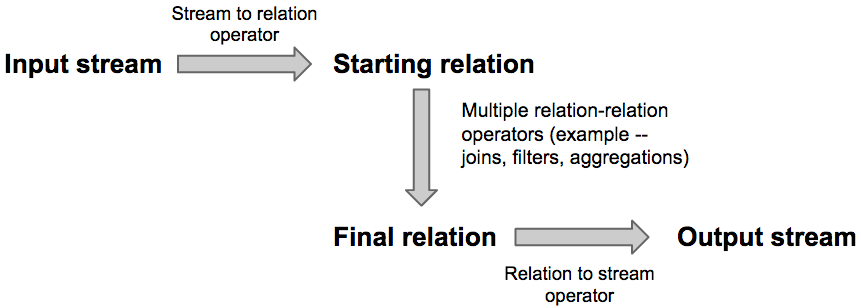
\includegraphics[totalheight=2.5cm]{operators.png}}
    \caption{Figure showing how a query that takes a stream as input and emits a stream as output is executed under the hood.}
    \label{fig:operators}
\end{figure}

We will revisit this model when we are considering actual SimpleCQL queries that we wrote to benchmark our implementation.


%%%%%%%%%%%%%%%%%%%%%%%%%%%%%%%%%%%%%%%%%%%%%%%%%%%%%%%%%%%%%%%%%%%%%%%%%%%%%%%%
\section{Implementation}
SimpleCQL is built on top of SimpleDB, a lightweight database implemented in Java. The \textit{relation} data primitive is already well-defined in SimpleDB, as are all of the Relation-to-Relation converters. As such, we only need to augment SimpleDB with implementations of the \textit{stream} data primitive, Stream-to-Relation operators, and Relation-to-Stream operators to fully support stream processing in SimpleCQL. 

\subsection*{Discretized Time}
SimpleCQL introduces a discretized notion of time in order to process continuous streams. Our system maintains an internal \textit{timestep} that is used to label tuples from continuous streams. This \textit{timestep} assignment does not correlate directly to cpu-time, application-time, or real-time, but serves to preserve the relative time ordering of incoming data. We require such an ordering to reason about and operate on tuples and relations in our concrete semantics.

The internal \textit{timestep} is updated each time our operators are invoked to consume from an input stream or emit to an output stream. Each update to \textit{timestep} represents the passage of one unit of discretized time -- our input and output streams also use this notion of discretized time. 

\subsection{Stream Readers}
A \textit{StreamReader} is an implementation construct we developed to represent an abstract \textit{stream} primitive. \textit{StreamReaders} allow us to discretize timesteps and read incoming tuples from an otherwise amorphous stream of data.

We implemented a generic StreamReader interface -- specific types of StreamReaders need to implement this interface. All StreamReaders need to implement a getNext(int timestep) function -- this function throws an exception if the requested timestep is too far out in the future, otherwise returns the next tuple that appears at that timestep (null if no such tuple exists).

We will now discuss two specific StreamReaders we implemented that are interesting, and relevant to the results presented later in this paper.

\begin{itemize}
\item \textbf{FileStreamReader}: This StreamReader reads a static file that is not changing to produce a stream -- each line in this static file is associated with a user-specified timestep, and the FileStreamReader will make these tuples ready to be consumed by downstream jobs at that specified timestep.
The implementation of this StreamReader is very simple -- the entire file is read into memory at initialization, and a map of timesteps to array of tuples is created. Once this is created, we can answer queries for tuples at any timestamp.

\item \textbf{LiveStreamReader}: This StreamReader tries to mimic tuples coming into the system in real time. A python script is used to produce a steady stream of tuples into a file; our LiveStreamReader then polls this file at regular intervals of time, reads in the new tuples written to the file by the Python script, and then makes these new tuples available to downstream jobs.
Our LiveStreamReader discretizes continuous time -- the time interval associated with a single timestep is configurable. In addition, to ensure that we have seen all tuples associated with a particular timestep $ts$, we need to see at least one tuple with timestep $ts + 1$.
\end{itemize}


\subsection{Stream-to-Relation Converters}
We implemented both a time-based Stream-to-Relation converter and a tuple-based Stream-to-Relation converter. 

\begin{itemize}

\item \textbf{Time-based Stream-to-Relation Converter:} The time-based converter is parameterized by a \textit{stream}, which is the input data source, and a \textit{windowSize}, which is the number of most recent timesteps to window the stream per advance in unit time. A time-windowed relation at $t = \tau$ with $windowSize = w$ will include all tuples from the stream with time labels $\in [\tau - w, \tau]$. The converter maintains the time-windowed relation as a list of tuples, and this data structure is initialized to be empty until consumption from the stream begins. We invoke the converter once to consume one timestep from the stream and incrementally update the internal relation data structure, adding only the new tuples that enter the window and removing only the old tuples that leave the window. Repeated invocation simulates the continuous forward motion of discretized time. Figure~\ref{fig:time_window} illustrates the relation data structure state with the passage of time. 

\begin{figure}[tpH]
    \centering
    \centerline{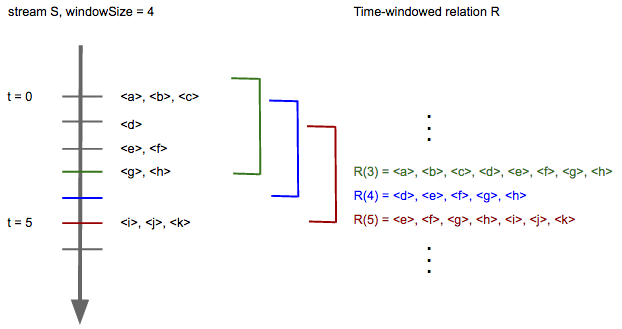
\includegraphics[totalheight=4cm]{time_window.png}}
    \caption{Example time-based Stream-to-Relation converter: windowed relation at three consecutive discretized timesteps with $windowSize = 4$.}
    \label{fig:time_window}
\end{figure}

\item \textbf{Tuple-based Stream-to-Relation Converter:} The tuple-based converter is similarly parameterized by a \textit{stream} and a \textit{tupleCount}, which is the number of most recent tuples to include per advance in unit time. A tuple-windowed relation at $t = \tau$ with $tupleCount = c$ will include the most recent $c$ tuples from the stream since time $\tau$. We similarly invoke the converter to incrementally consume one timestep from the stream, adding the tuples at the new timestep and removing old tuples until the relation size is $c$. Figure~\ref{fig:tuple_window} illustrates the relation data structure with the passage of time. 

\begin{figure}[tpH]
    \centering
    \centerline{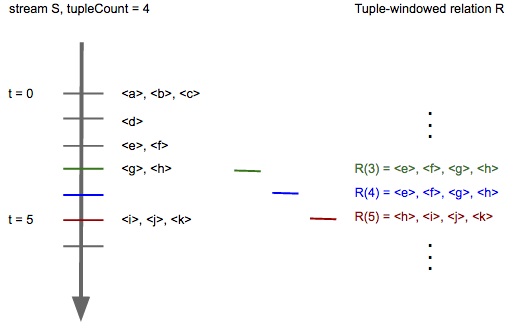
\includegraphics[totalheight=4cm]{tuple_window.png}}
    \caption{Example tuple-based Stream-to-Relation converter: windowed relation at three consecutive discretized timesteps with $tupleCount = 4$.}
    \label{fig:tuple_window}
\end{figure}
\end{itemize}

Both converters return, per advancing timestep, a \textit{DbIterator} of the windowed relation that is compatible with existing relational operators in SimpleDB.

\subsection{Relation-to-Stream Converters}
The Relation-to-Stream converters are similar to the Stream-to-Relation converters in that they are also repeatedly invoked to simulate the continuous forward motion of discretized time. Relation-to-Stream converters generate an output \textit{stream}; each update invocation takes in a relation at time $t = \tau$ and compares it to the previous input relation at time $t = \tau - 1$, emitting the corresponding tuples to the output stream. 

\begin{itemize}
\item \textbf{Insertion Stream:} The Insertion Stream emits to the output stream all of the tuples that are present in the new $relation_{\tau}$ but that were not present in the previous $relation_{\tau - 1}$. Thus, IStream($\tau$) can be generalized to be defined as $relation_{\tau} -relation_{\tau - 1}$.

\item \textbf{Deletion Stream:} The Deletion Stream emits all tuples that are not present in the new $relation_{\tau}$ but that were present in the previous $relation_{\tau - 1}$. Dstream($\tau$) is defined as $relation_{\tau - 1} - relation_{\tau}$.

\item \textbf{Relation Stream:} The Relation Stream emits at time $t = \tau$ all tuples in the $relation_{\tau}$ that is passed into the converter update. RStream($\tau$) is exactly $relation_{\tau}$.
\end{itemize}

We implement these diffs-based computations by maintaining the $prevRelation$, hashing the tuples of $prevRelation$, and then probing into the hash set with tuples of $nextRelation$ to determine the differences across timesteps. Figure Z illustrates the emitted tuples for each of the Relation-to-Stream converters with respect to time; the IStream is highlighted because it is most illustrative and most significant in our system. 

\begin{figure}[tpH]
    \centering
    \centerline{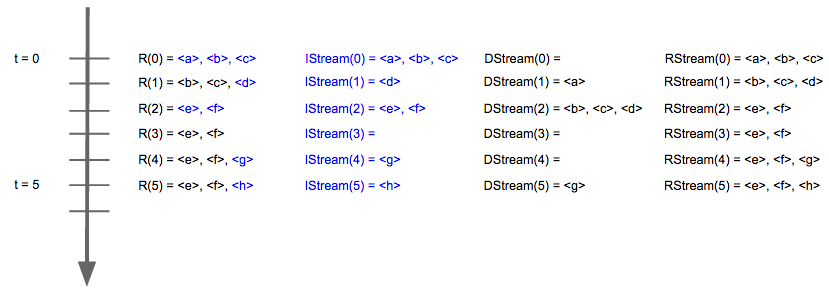
\includegraphics[totalheight=3cm]{stream_converter.png}}
    \caption{Changes in the input Relation $R$ over time and the corresponding updates to IStream, Dstream, and RStream.}
    \label{fig:stream_converter}
\end{figure}


\subsection{Garbage Collection}
We implemented garbage collection in our system to ensure that streams aren’t stored in their entirety at any point in time -- this is desirable since streams can become arbitrarily large, especially if tuples are accumulated for a long time.

Two possible garbage collection policies are possible -- a time based garbage collection policy, where tuples from too far out in the past are discarded (this is suitable for queries featuring streams that are windowed using a time-based Stream-to-Relation converter) and a tuple based garbage collection policy, where tuples are discarded once the number of tuples in the system passes a certain threshold.

For now, we have only implemented the time based garbage collection policy. Effects on memory footprint and performance are talked about in the performance portion of this paper.


%%%%%%%%%%%%%%%%%%%%%%%%%%%%%%%%%%%%%%%%%%%%%%%%%%%%%%%%%%%%%%%%%%%%%%%%%%%%%%%%
\section{Evaluation}
Benchmarks of SimpleCQL were performed on an AWS Compute Optimized (c3.8xlarge) instance with 60 GiB of memory, 32 vCPUs, 640 GB of SSD-based local instance storage, and a 64-bit platform.  When applicable, SimpleCQL performance was compared to that of SimpleDB and the continuous workload of SimpleCQL is shown to outperform equivalent discretized workloads of SimpleDB.  

\subsection{Testing Conditions}
SimpleDB was intended to be a toy database designed for teaching core concepts of database internals.  As such, the performance of both SimpleDB and SimpleCQL suffer from a lack of optimizations.  However, a pairwise comparison uses the same underlying operations and care was taken to keep comparison even, i.e. SimpleDB never wrote tuple insertions to disk.

SimpleDB's code is largely unoptimized, so the SimpleCQL performance metrics we present in this paper can be greatly improved upon using standard optimization techniques prevalent in the literature. 

Many of the benchmark tests were run over $D = 1800$ timesteps and the number of tuples per timestep $R$ was increased to measure performance.  Equation ~\ref{eq:throughput} is used to estimate the projected throughput of the system.

\begin{equation} \label{eq:throughput}
    \text{Throughput} = R \text{ tuples/timestep} \times \dfrac{D \text{ timesteps}}{T \text{ seconds}}
\end{equation}


TODO: Note that file reading was not accounted for in execution time.

We didn't use B+Trees, and other optimizations built into SimpleDB because we wanted to do an apples-apples comparison, and wanted to measure the gain produced from our windowing strategy alone.

\subsection{Log Analysis: Detecting Attacks}
Most web companies wish to keep their users accounts safe and out of reach of hackers and spammers.  On occasion though, hackers obtain lists of potentially millions of usernames.  These users can then be victims of a brute-force attack, where attackers try to brute force through all possible strings to guess a user'��s password. This leads to a spike in the number of failed login attempts. Access to real-time error log statistics allows spam and abuse teams to easily detect such an attack and respond as necessary.

In this example, we consider a stream of log messages, \texttt{LogStream}. We formally define the schema of the stream as: \texttt{LogStream\{Message:STRING\}}. Given this schema, a rolling count of log messages that contain the string ``failed login" provides the relevant information for the above situation.  The following query computes a rolling count of failed login attempts.

\begin{lstlisting}
SELECT ISTREAM(
    count(*)
)
FROM LogStream [Range 1 second]
WHERE LogStream.Message
	LIKE "%failed login%"
GROUP BY LogStream.Message;
\end{lstlisting}

Data for the \texttt{LogStream} was generated prior to running tests and read using a custom \texttt{FileStreamReader}.  The data generated represents 30 minutes of log messages.

\begin{figure}[tpH!]
    \centering
    \centerline{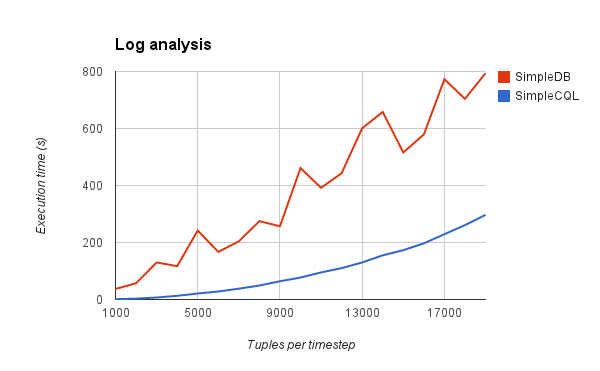
\includegraphics[totalheight=5cm]{attack.png}}
    \caption{Performance of SimpleDB and SimpleCQL detecting attacks.}
    \label{fig:attack}
\end{figure}

As seen in Figure~\ref{fig:attack}, SimpleCQL drastically outperforms SimpleDB when running queries over relatively small time windows (several seconds).  As the number of tuples per timestep is increased, the difference in execution time between SimpleCQL and SimpleDB also increased.  

SimpleCQL was able to achieve about an order of magnitude speedup over SimpleDB.  The projected throughput of SimpleCQL is approximately 400k tuples/second, whereas the projected throughput of SimpleDB is approximately 50k tuples/second.

\subsection{Trending Tweets}
Trending tweets on Twitter are useful for a variety of reasons.  The company may use them to increase user engagements, optimize advertisements, or analyze the state of current events.  

In this example, we consider a stream of Twitter tweets, \texttt{TweetStream}. We formally define the schema of the stream as: \texttt{TweetStream\{Text:STRING, Hashtag:STRING, Location:STRING\}}.  Given this schema, a rolling count of log messages that contain the string ``failed login" provides the relevant information for the above situation.  The following query computes the rolling count.

\begin{lstlisting}
SELECT ISTREAM(
    TweetStream.Hashtag,
    MAX(COUNT(*))
)
FROM TweetStream [Range 30 seconds]
WHERE TweetStream.Location = "Boston"
GROUP BY TweetStream.Hashtag;
\end{lstlisting}

Data for the \texttt{TweetStream} was generated prior to running tests.  The data generated represents 30 minutes of tweets with text, hashtags, and locations.   

\begin{figure}[tpH!]
    \centering
    \centerline{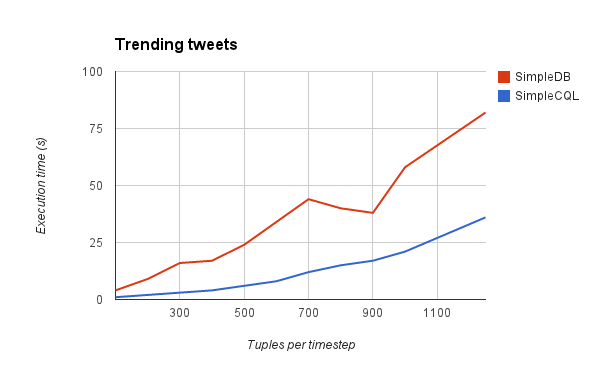
\includegraphics[totalheight=5cm]{trending.png}}
    \caption{Performance of SimpleDB and SimpleCQL calculating trending tweets.}
    \label{fig:trending}
\end{figure}

As seen in Figure~\ref{fig:trending}, SimpleCQL again outperforms SimpleDB when running queries over larger time windows.  As the number of tuples per timestep is increased, the difference in execution time between SimpleCQL and SimpleDB also increased.

The projected throughput of SimpleCQL is approximately 100k tuples/second, whereas the projected throughput of SimpleDB is approximately 35k tuples/second.

\subsection{Advertisement Statistics}
The Advertising Statistics example, presented in detail in section 2, involves joining advertisement insertions across two disparate streams.  Specifically a stream of advertisement insertions, known as \texttt{InsertionStream}, and a stream of advertisement events, known as \texttt{EventStream}, are joined on \texttt{InsertionId} in order product real-time per-advertisement click-through rate.  The following query computes the join.

\begin{lstlisting}
SELECT RSTREAM (
    advertisement_id,
    SUM(type = 'click' ? 1 : 0) / 
    SUM(type = 'impression' ? 1 : 0)
)
FROM (
    SELECT ISTREAM(advertisement_id, type)
    FROM InsertStream [Range 600 seconds], 
         EventStream [Range 1 second] 
    WHERE InsertStream.insertion_id = 
    EventStream.insertion_id
) 
GROUP BY advertisement_id;
\end{lstlisting}

Data for the \texttt{InsertionStream} and \texttt{EventStream} was generated prior to running tests.  The data generated represents 30 minutes of advertisement insertions.  Each insertion in the \texttt{InsertionStream} may have a corresponding impression and click event in the EventStream that appears up to 10 minutes after the insertion.

\begin{figure}[tpH!]
    \centering
    \centerline{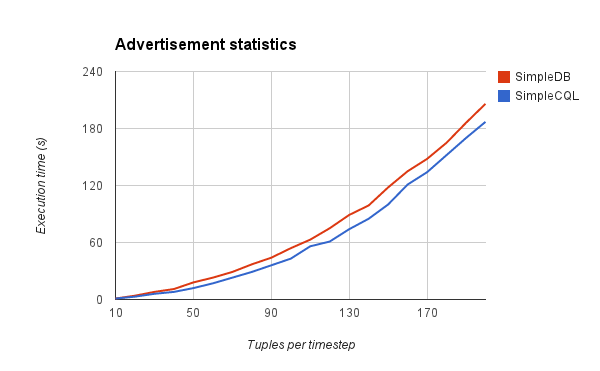
\includegraphics[totalheight=5cm]{ads.png}}
    \caption{Performance of SimpleDB and SimpleCQL computing real-time click-through rates.}
    \label{fig:ads}
\end{figure}

\begin{figure}[tpH!]
    \centering
    \centerline{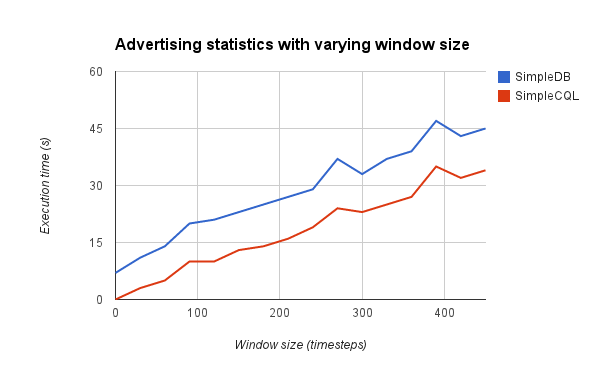
\includegraphics[totalheight=5cm]{ads_window.png}}
    \caption{Performance of SimpleDB and SimpleCQL computing real-time click-through rates with varying window.}
    \label{fig:ads_window}
\end{figure}

As seen in Figure~\ref{fig:ads}, SimpleCQL does not notably outperform SimpleDB when running queries over very large time windows with complex queries.  It is important, however, that SimpleCQL did not degrade and 

The projected throughput of SimpleCQL is approximately 8k tuples/second, whereas the projected throughput of SimpleDB is approximately 6.5k tuples/second.  Both systems are severely hindered by a very large unoptimized nested-loop join running at every timestep.

\subsection{Garbage Collection}
As expected Garbage collection drastically reduced the memory footprint of the system, but reduced performance slightly. These points are better illustrated in the following graphs, which were produced using our LiveStreamReader.

\begin{figure}[tpH!]
    \centering
    \centerline{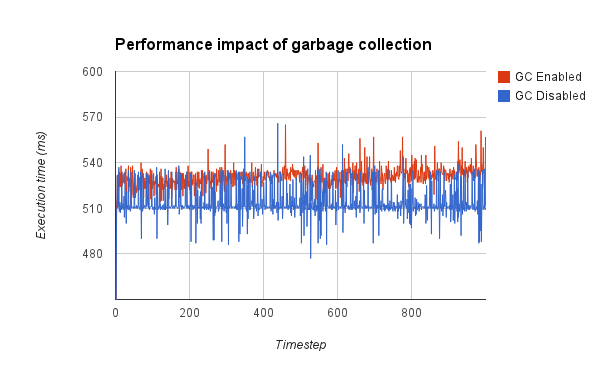
\includegraphics[totalheight=5cm]{gc_perf.png}}
    \caption{Plot of execution time per timestamp versus timestamp with and without garbage collection. With Garbage Collection enabled, the system performs marginally worse than with Garbage Collection disabled}
    \label{fig:gc_perf}
\end{figure}

%%%%%%%%%%%%%%%%%%%%%%%%%%%%%%%%%%%%%%%%%%%%%%%%%%%%%%%%%%%%%%%%%%%%%%%%%%%%%%%%
\section{Conclusion}
*note: be explicit about how the goal is to support stream processing using traditional SQL-like semantics/relational operators. We have motivated the need for a continuous query language, shown the meaning of a ``continuous query language" through abstract semantics, and built a system that supports a large variety of complex queries.  Our system performs very well and has much room for improvement and optimizations.  TODO.

%%%%%%%%%%%%%%%%%%%%%%%%%%%%%%%%%%%%%%%%%%%%%%%%%%%%%%%%%%%%%%%%%%%%%%%%%%%%%%%%
\bibliographystyle{plain}
\bibliography{references}


\end{document}
